%\documentclass[conference]{IEEEtran}
\documentclass[journal,onecolumn,12pt]{IEEEtran}

\usepackage{graphicx}
\usepackage{bm}% bold math

\usepackage{epsfig}

%\usepackage{cite}
%\usepackage[bookmarks=true,pdfstartview=FitH]{hyperref}
\usepackage[bookmarks=true,pdfstartview=FitH,,bookmarksopen=true,colorlinks,citecolor=blue,filecolor=green,linkcolor=blue,urlcolor=blue]{hyperref}
\usepackage{bookmark}

\usepackage{algpseudocode}
\usepackage{algorithm}

\usepackage[caption=false]{subfig}
%\usepackage{fixltx2e}
\usepackage{stfloats}
\usepackage{url}
\usepackage{multirow}
\usepackage{threeparttable}

% correct bad hyphenation here
\hyphenation{op-tical net-works semi-conduc-tor}

\begin{document}

\title{Energy-efficient and Cross-layer Networking in Mobile MIMO-OFDM Systems}

\author{\IEEEauthorblockN{Yongsen MA} \\
\IEEEauthorblockA{Shanghai Jiao Tong University \\
E-mail: mayongsen@gmail.com}
}

% make the title area
\maketitle
%
%\begin{abstract}
%%\boldmath
%The abstract goes here.
%\end{abstract}


\section{Statement of Purpose}
The wireless networks such as LTE, WiMAX, WLAN have experienced rapid development in recent years, which leads to the increase of traffic loads and users requirements. The wide expansion of wireless services has brought serious challenges to the issues of spectrum efficiency.

As demand for more powerful hardware, more advanced software, and constant data connections grows larger, the need for a more efficient and longer lasting mobile battery is becoming increasingly vital to the future of the industry.

\subsection{Traffic Requirements}
\begin{figure}
\centering
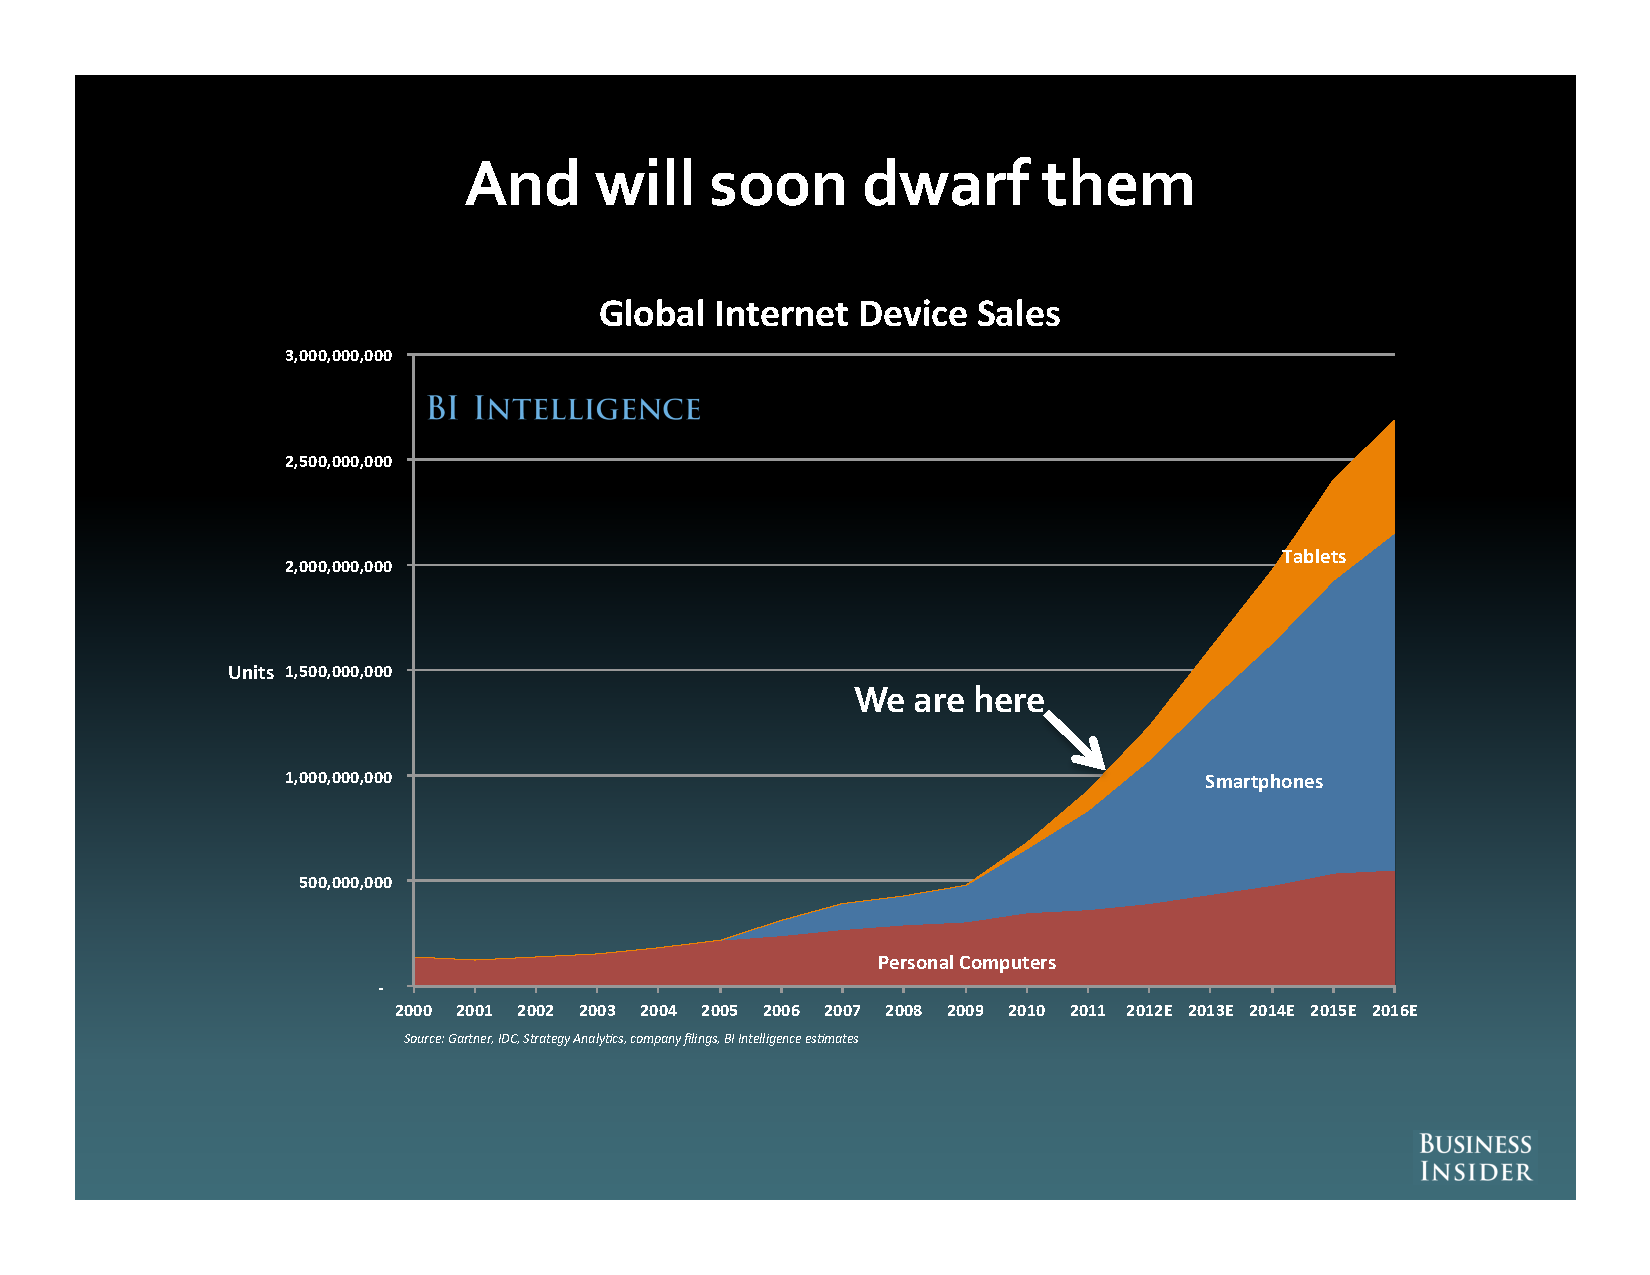
\includegraphics[width=0.8\textwidth]{device_trend.pdf}
\caption{Global Internet Device Sales.}
\label{fig:device_trend}
\end{figure}

\begin{figure}
\centering
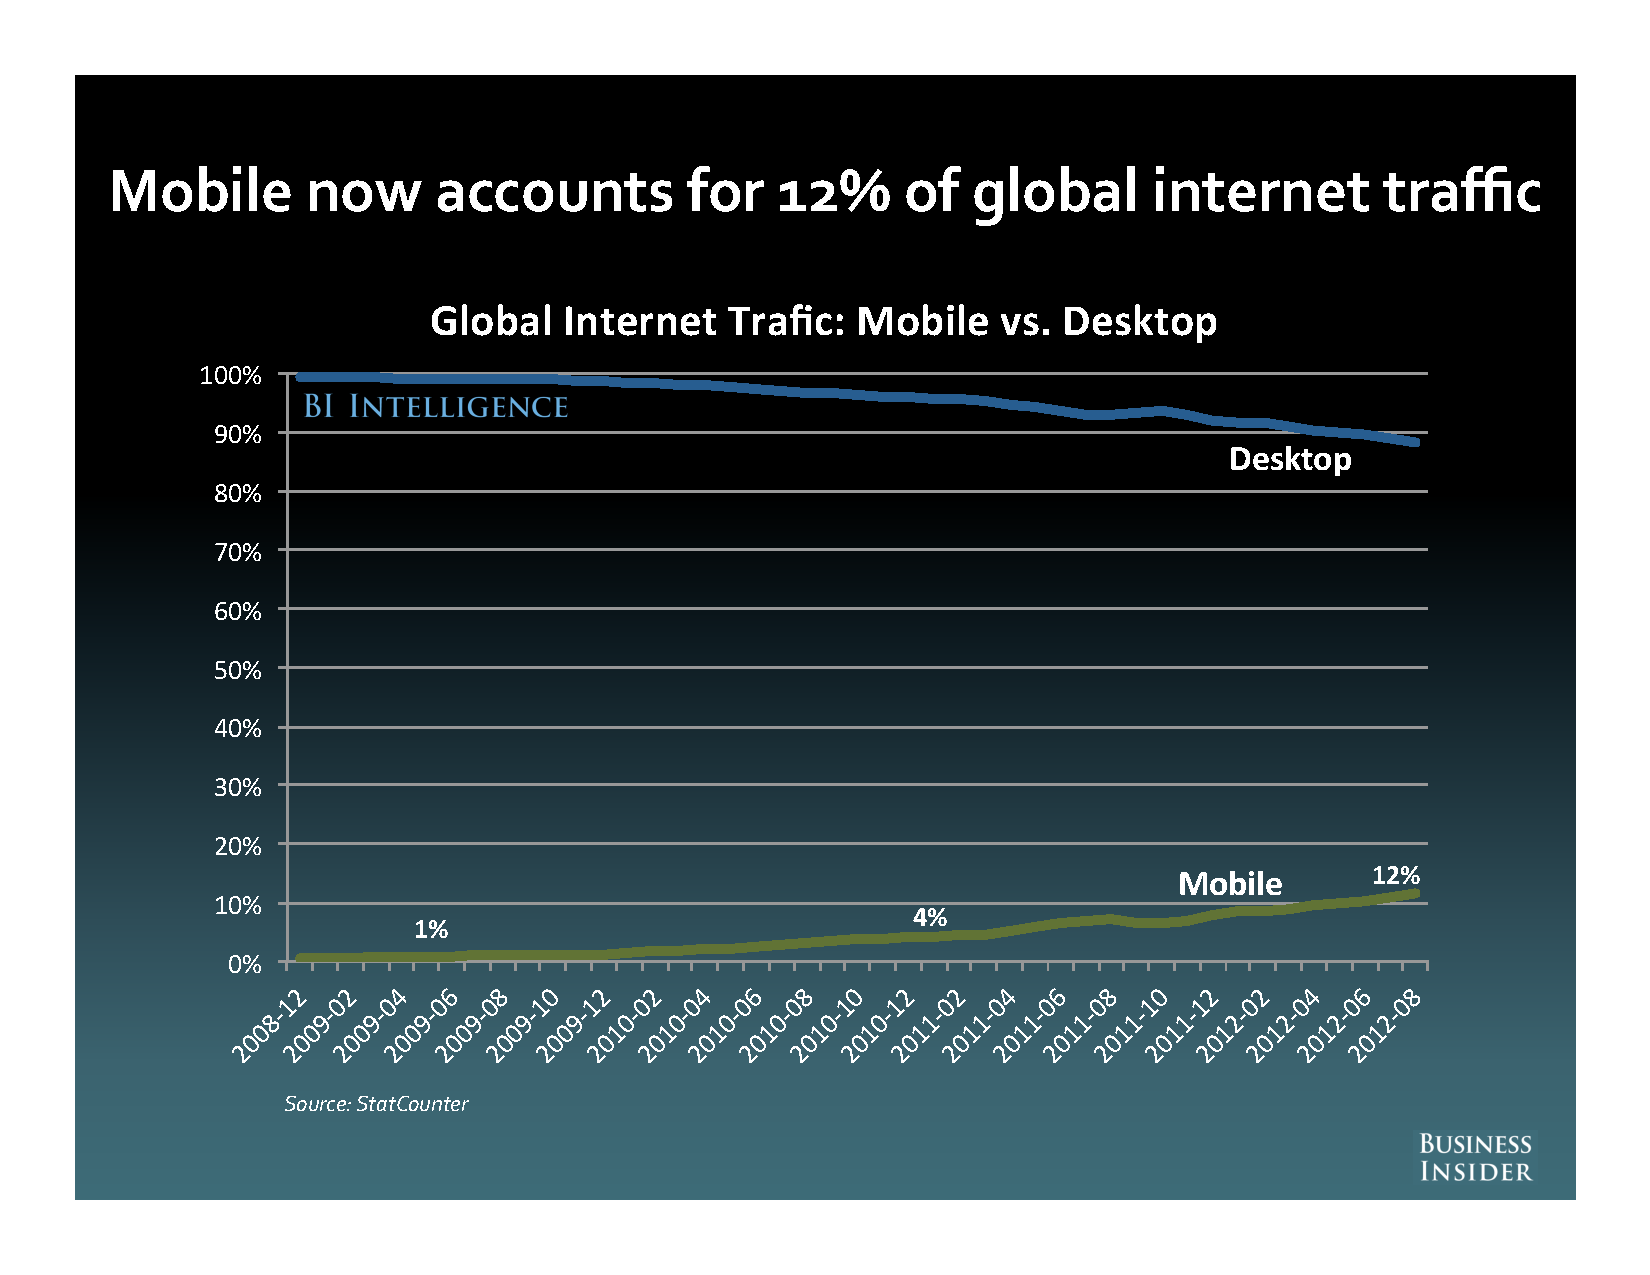
\includegraphics[width=0.8\textwidth]{mobile_desktop.pdf}
\caption{Global Internet Traffic: Mobile vs. Desktop.}
\label{fig:mobile_desktop}
\end{figure}

\begin{figure}
\centering
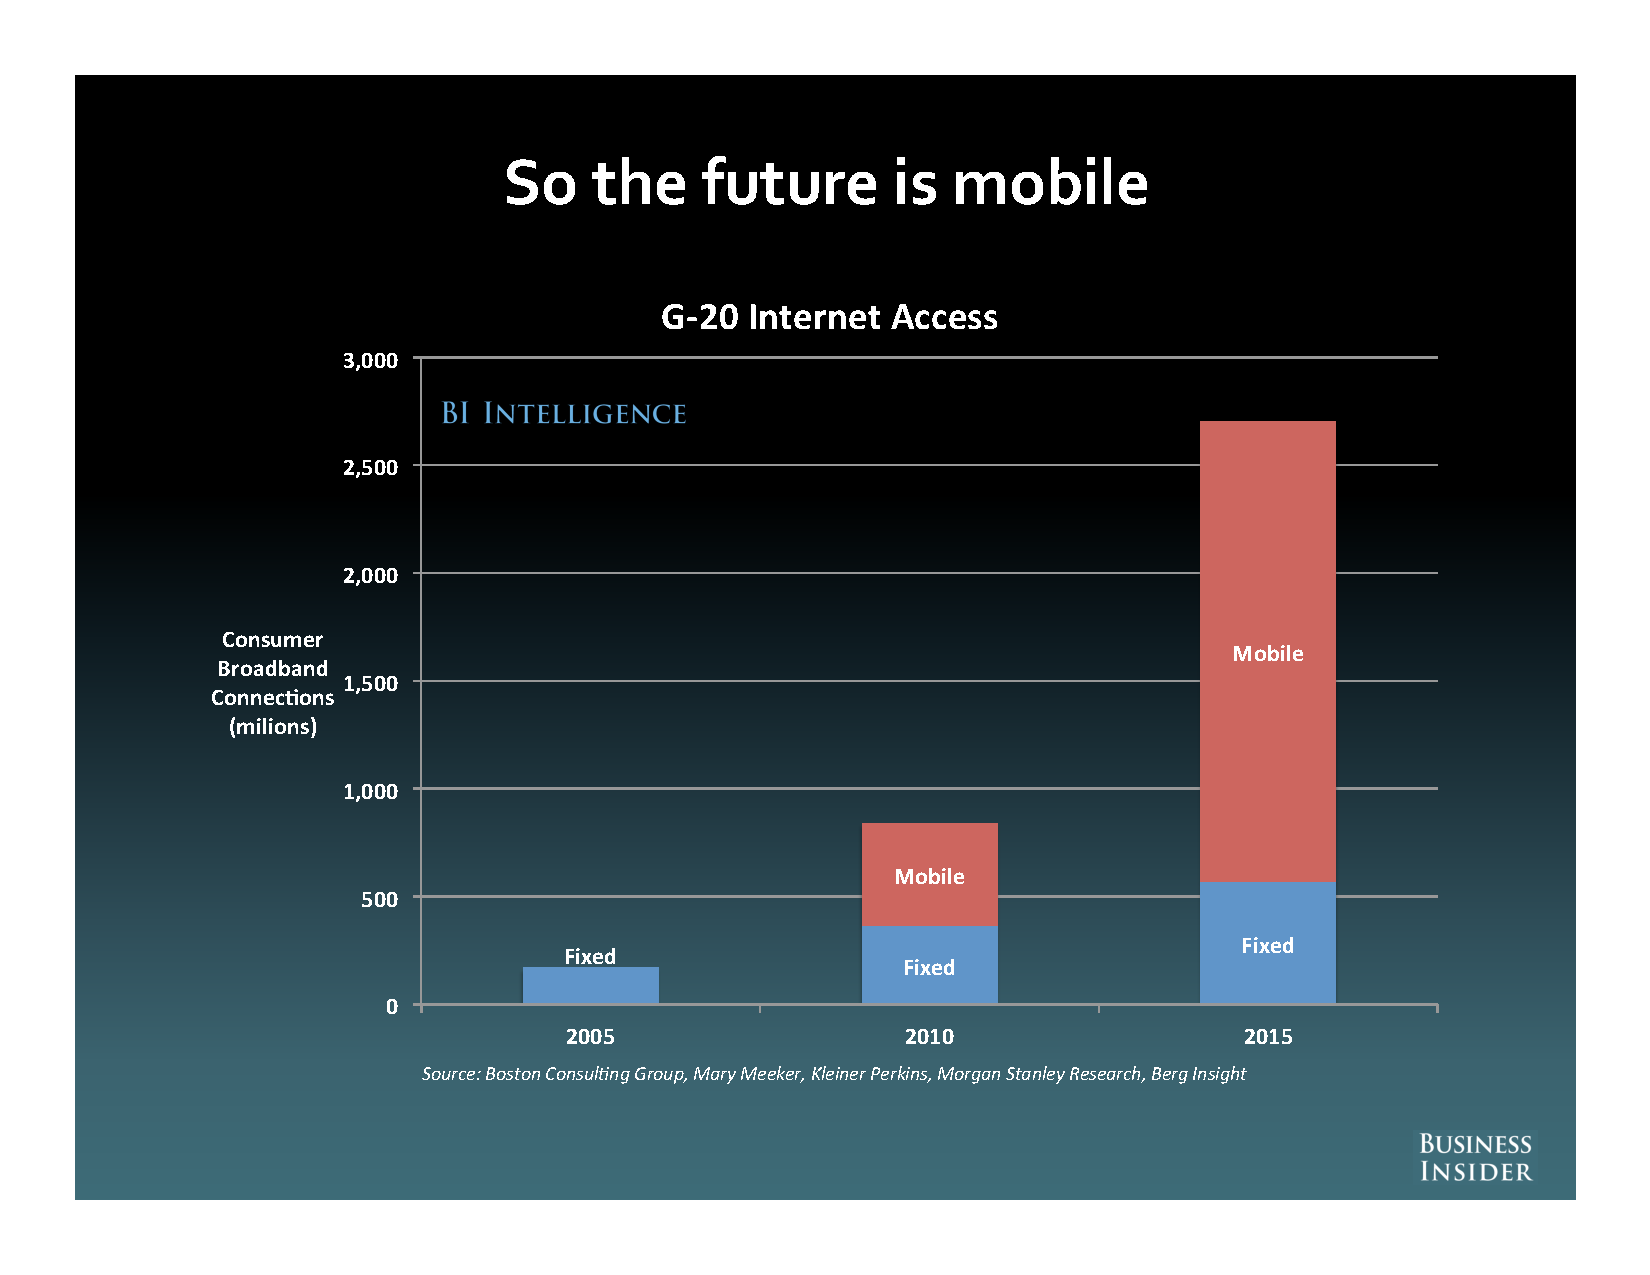
\includegraphics[width=0.8\textwidth]{mobile_trend.pdf}
\caption{Internet Access: Mobile vs. Fixed.}
\label{fig:mobile_trend}
\end{figure}

\begin{figure}
\centering
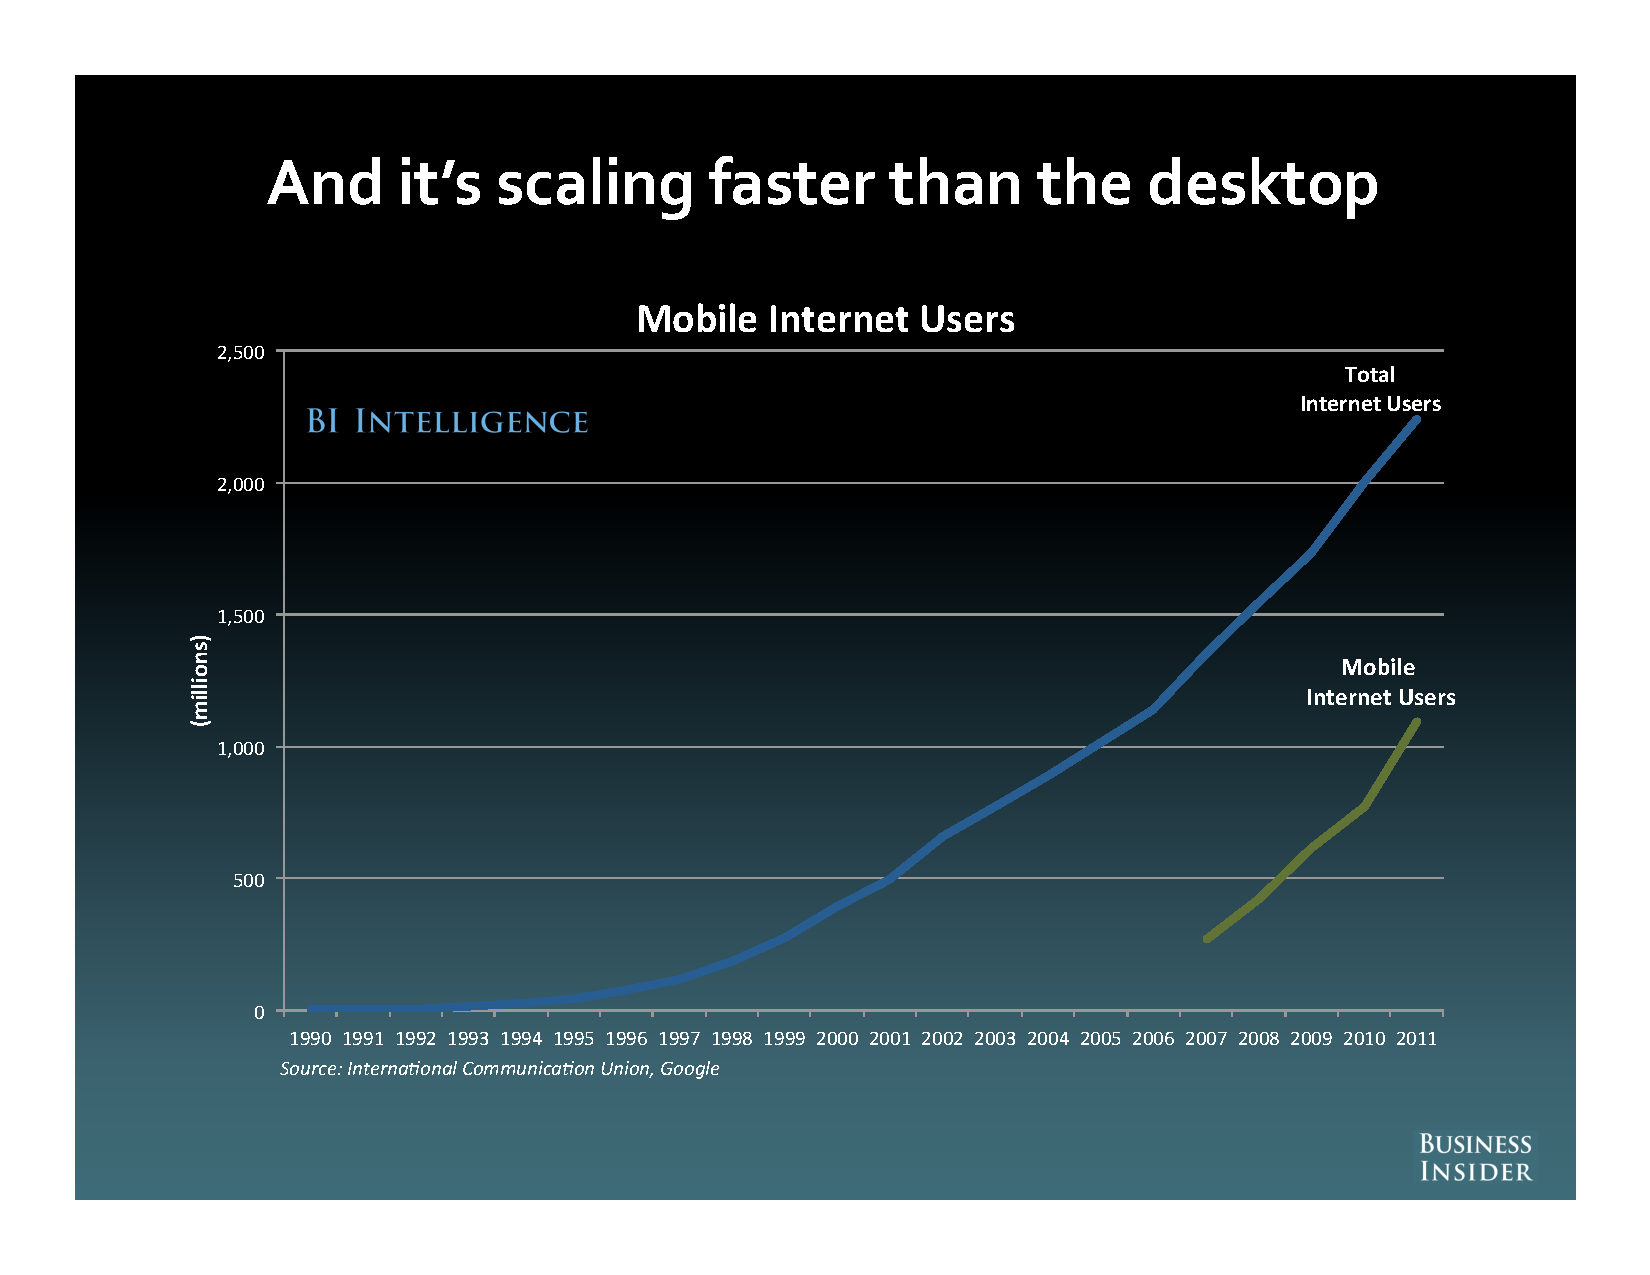
\includegraphics[width=0.8\textwidth]{mobile_users.pdf}
\caption{Mobile Internet Users.}
\label{fig:mobile_users}
\end{figure}

\subsection{Spectrum Efficiency}

\subsection{Energy Efficiency}

\section{Research Questions}
These should be framed as questions, or hypotheses. They should not be statements or descriptions. Here are some examples for phrasing questions:
\begin{itemize}
  \item What are the major determinants of women's success in the job market?
  \item Why are there variations in women's earnings across three provinces?
  \item What does the changing role of gender play in early 20th century Chinese fictions?
\end{itemize}

\begin{enumerate}
  \item System level
  \item Protocol level
\end{enumerate}

\section{Literature Review}
Say how other scholars have tried to answer the questions that you mention above. The literature review must be
relevant to the questions you are asking. For example, if you want to know how women's lives have changed as
a result of starting a business in China, you do not need to review all the literature on China's political and
economic reforms. Instead, you want to locate the literature on how women's lives are affected by the
development of market economies.

\section{Statement of Significance}
Think about the overall implications of your work. Look beyond how undertaking the degree will help you
personally. PhD or MPhil theses may have several implications. Consider the following:
\begin{enumerate}
  \item They may contribute to a body of academic literature. They may, for instance, advance a neglected theoretical
position.
  \item They may have practical or policy implications. For example, they may change the way that a certain group
of people practice their occupation, handle their clients or deal with their work.
  \item They may make a political statement or a cultural critic. They may point to an injustice, an inequality, or a
contradiction.
\end{enumerate}

But be realistic. It is not realistic to claim that your work will, say, transform the educational system in Hong
Kong. It may be realistic, however, to say that your thesis will help explain why students often fail to live up to
teachers' expectations.

\section{Research Methodology}
Research methodology concerns the manner by which data are collected. Documentation, observation, in-depth
interview, survey, and statistical data are the main methods of data collection in the social sciences.

Your methodology must be  appropriate  to the questions you are asking. That is, you must show how the
methods you use will answer the questions you are asking. If you want to study recreational drug use in Hong
Kong, for example, it would not be appropriate to study only youth in your housing estate who do not take drugs.

Further, your methodology must be feasible. A proposal to interview workers from 500 factories in Shenzhen is
not feasible--in the time that you have to complete the degree. It may, however, be feasible to interview workers
from ten factories, or obtain production statistics from 500 enterprises.

Finally, your methodology must be detailed. For example, if you plan to do a survey, how many people do you
plan to include in your sample? And how will you decide which people to sample?

\nocite{*}

\renewcommand\refname{References}
\bibliographystyle{abbrv}
%\IEEEtriggeratref{6}
\bibliography{wireless}
%\printbibliography

\end{document}
